\documentclass{article}
\usepackage{graphicx}
\usepackage{fontspec}
\usepackage{fancyvrb}
\usepackage{booktabs}

\setsansfont{Latin Modern Sans}
%\usepackage[math-style=ISO,bold-style=ISO]{unicode-math}
\usepackage{xunicode}
\usepackage{fontspec}
\defaultfontfeatures{Mapping=tex-text}
\usepackage{libertine}
%\setmainfont{Linux Libertine O}
\setsansfont{Linux Biolinum O}
%\setmonofont{Inconsolata}
%\setmathfont{XITS Math}

\usepackage[a4paper]{geometry}
\author{Laurent George}
\title{Heuristic analysis}
\begin{document}
\maketitle

\section{Evaluation heuristics}

The following evaluation heuristics were implemented:

\begin{description}
    \item[Combined:] Combination of improved heuristics and density. The objective is to look for positions that are located in low density area. To limit time impact of computing density, the density function is only used if the number of moves is above 20 (i.e when we are approaching the end of the game).
\item[Diff\_density:] Difference in number of free space around player and opponent. It allows to prefer to go to places where there are a lot of free spaces.
%\item[Improved Agressive heuristic:] An heuristic that priviledge the attack.
\item[Slow:] Similar to ID\_Improved but penalised with a sleep of 10ms. The objective is to measure the impact of a slow heuristic.
\item[Distance:] The score is based on l1-norm (taxicab distance) between player and the board center. The objective is to encourage position near the center of the board.
\end{description}

\section{Results}

\emph{Tournament.py} was used to run the evaluation of heuristics (raw output is provided in section~\ref{annexe1}). 
The analysis was run with the variable \emph{NUM\_MATCHES} set to 100 to get 400 games per opponent. This allowed to have more accurate results. To accelerate the evaluation process the Python multiprocessing library was used. Thus allowing to run the matches on 4~CPU core at the same time. The six default opponents (\emph{Random},  \emph{MM\_Null},  \emph{MM\_Open},  \emph{MM\_Improved}, \emph{AB\_Null}, \emph{AB\_Open}, \emph{AB\_Improved}) were used.

\begin{table}
    \centering
\begin{tabular}{lr}
\toprule
{} &           winning rate \\
\midrule
    Combined     &   \bf{77.57}\% \\
    Diff\_density &    74.32\% \\
    Distance     &   70.39\% \\
    ID\_Improved &     74.86\% \\
    Slow         &   32.07\% \\
\bottomrule
\end{tabular}
    \caption{Average wining rate for the different heuristics \label{table:percentage}}
\end{table}
\clearpage

Table~\ref{table:percentage} show the average winning rate of each heuristic. The \emph{Combined} evaluation heuristic provides the best average winning rate (77.57\%) which is 3.25\% better than the \emph{ID\_Improved} heuristic. The Slow heuristic has the lowest score. This highlights the impact of a slow heuristic, and it could be explained by the fact that the \emph{Slow} heuristic does not allow to reach high depth due to timeout.


Table~\ref{table:detail_percentage} show the winning rate of each heuristic versus each opponent. \emph{Combined} heuristic is the winning heuristic here (5 out of 7 best results). 

As highlight in figure~\ref{fig:boxplot} the \emph{Combined} and \emph{ID\_improved} are the two heuristics that provide the lowest variation against opponents, thus we can consider them as the more stable. We can also observe that the four heuristics (\emph{Combined}, \emph{Diff\_density}, \emph{Distance}, \emph{ID\_Improved}) have close distributions in terms of winning rate.

\begin{table}
    \centering
\begin{tabular}{lccccc}
\toprule
 & Combined & Diff\_density & Distance & ID\_Improved &   Slow \\
        &          &              &          &             &        \\
\midrule
    AB\_Improved &   \bf{68.25\%} &       61.75\% &   54.00\% &      62.75\% & 17.75\% \\
    AB\_Null     &   78.50\% &       \bf{80.00\%} &   76.75\% &      79.00\% & 31.75\% \\
    AB\_Open     &   \bf{71.00\%} &       61.50\% &   64.00\% &      66.75\% & 21.75\% \\
    MM\_Improved &   \bf{70.25\%} &       66.00\% &   59.75\% &      68.00\% & 17.50\% \\
    MM\_Null     &   85.75\% &       \bf{86.75\%} &   83.25\% &      82.75\% & 44.75\% \\
    MM\_Open     &   \bf{75.00\%} &       71.50\% &   66.50\% &      72.00\% & 22.50\% \\
    Random      &   \bf{94.25\%} &       92.75\% &   88.50\% &      92.75\% & 68.50\% \\
\bottomrule
\end{tabular}
    \caption{Winning rates for each heuristic versus each opponent. Highest winning rates are highlighted in bold. \label{table:detail_percentage}}

\end{table}

\begin{figure}[h]
    \centering
    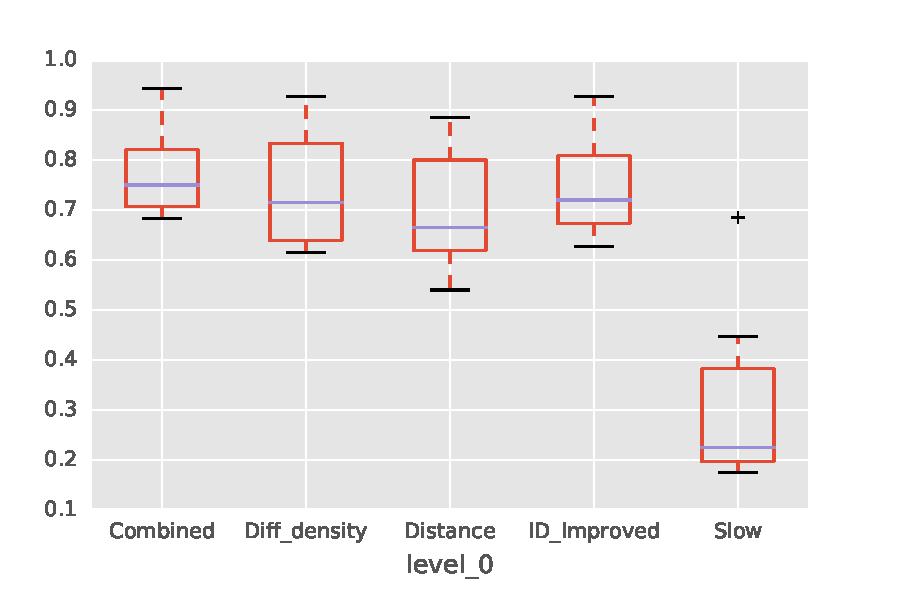
\includegraphics[width=0.75\textwidth]{boxplot.pdf}
    \caption{Box-plot for the different heuristics \label{fig:boxplot}}
\end{figure}

The results show that the \emph{Combined} heuristic offers the best results in terms of stability, average performance, and median performance, thus we can recommend its use as the default heuristic for the game. However, this recommendation should be taken with care as the improvement is low compared to \emph{ID\_Improved}, a better heuristic may exist but we did not find it.

\newpage
\section{Annexe}
\label{annexe1}

\VerbatimInput{data.txt}

\end{document}
